\chapter{INTRODUCCIÓN}

	\par Una red de computadoras es un conjunto de computadoras autónomas 
interconectadas. Dos computadoras están interconectadas si pueden intercambiar 
información. La conexión puede hacerse por medio de: cable de cobre, fibra óptica, 
microondas, rayos infrarrojos, satélites de comunicaciones, etc.

	\par Si bien los tipos de redes no cambian, si evoluciona la tecnología de hardware en 
la que se basa, y como consecuencia el funcionamiento o desempeño de las redes de 
cada tipo van mejorando más y más.

\section{Uso de las redes de las computadoras}
\par Aplicaciones de negocios
\par Aplicaciones domésticas
\par Usuarios móviles
\par Cuestiones sociales

\section{Hardware de red}
\par Dos tipos de tecnología de transmisión:
	\begin{itemize}
		\item Las redes de difusión tienen un solo canal de comunicación, por lo que 
		todas las máquinas de la red lo comparten.
		\item En las redes punto a punto un paquete podría tener que visitar una o más 
		máquinas intermedias. Puede haber varias rutas diferentes y hay que encontrar la 
		correcta.
	\end{itemize}
\par Las redes más pequeñas suelen usar difusión, mientras que las más grandes 
conectan redes pequeñas punto a punto.

\subsection{Redes de área local}
\par Las redes de área local, generalmente llamadas LAN (Local Area Networks), son 
redes de propiedad privada que operan dentro de un solo edificio, como una casa, 
oficina o fábrica.
\subsubsection{Difusión}
\par Si una máquina envía un mensaje todas las demás lo reciben, dentro del mensaje se indica el destinatario. Una máquina al recibir un paquete analiza si va destinado a ella y en ese caso lo procesa, sino lo ignora. Otras variantes son: \textit{broadcasting}, consiste en enviar un paquete a todos y \textit{multicasting} envia a un grupo particular.
\par Ejemplos de redes de área local son WIFI y Ethernet.

\par \textbf{WiFi:} son redes inalámbricas, operan a velocidades desde 11 hasta cientos de Mbps.

\par \textbf{Ethernet:} Son redes de difusión basada en bus con control descentralizado que funcionan de 10 Mbps a 10 Gbps. Se puede transmitir siempre que se desee; si dos paquetes colisionan, es decir mas de una máquina escribiendo simultáneamente en el cable, se espera un tiempo aleatorio e intenta más tarde.

\begin{center} 
	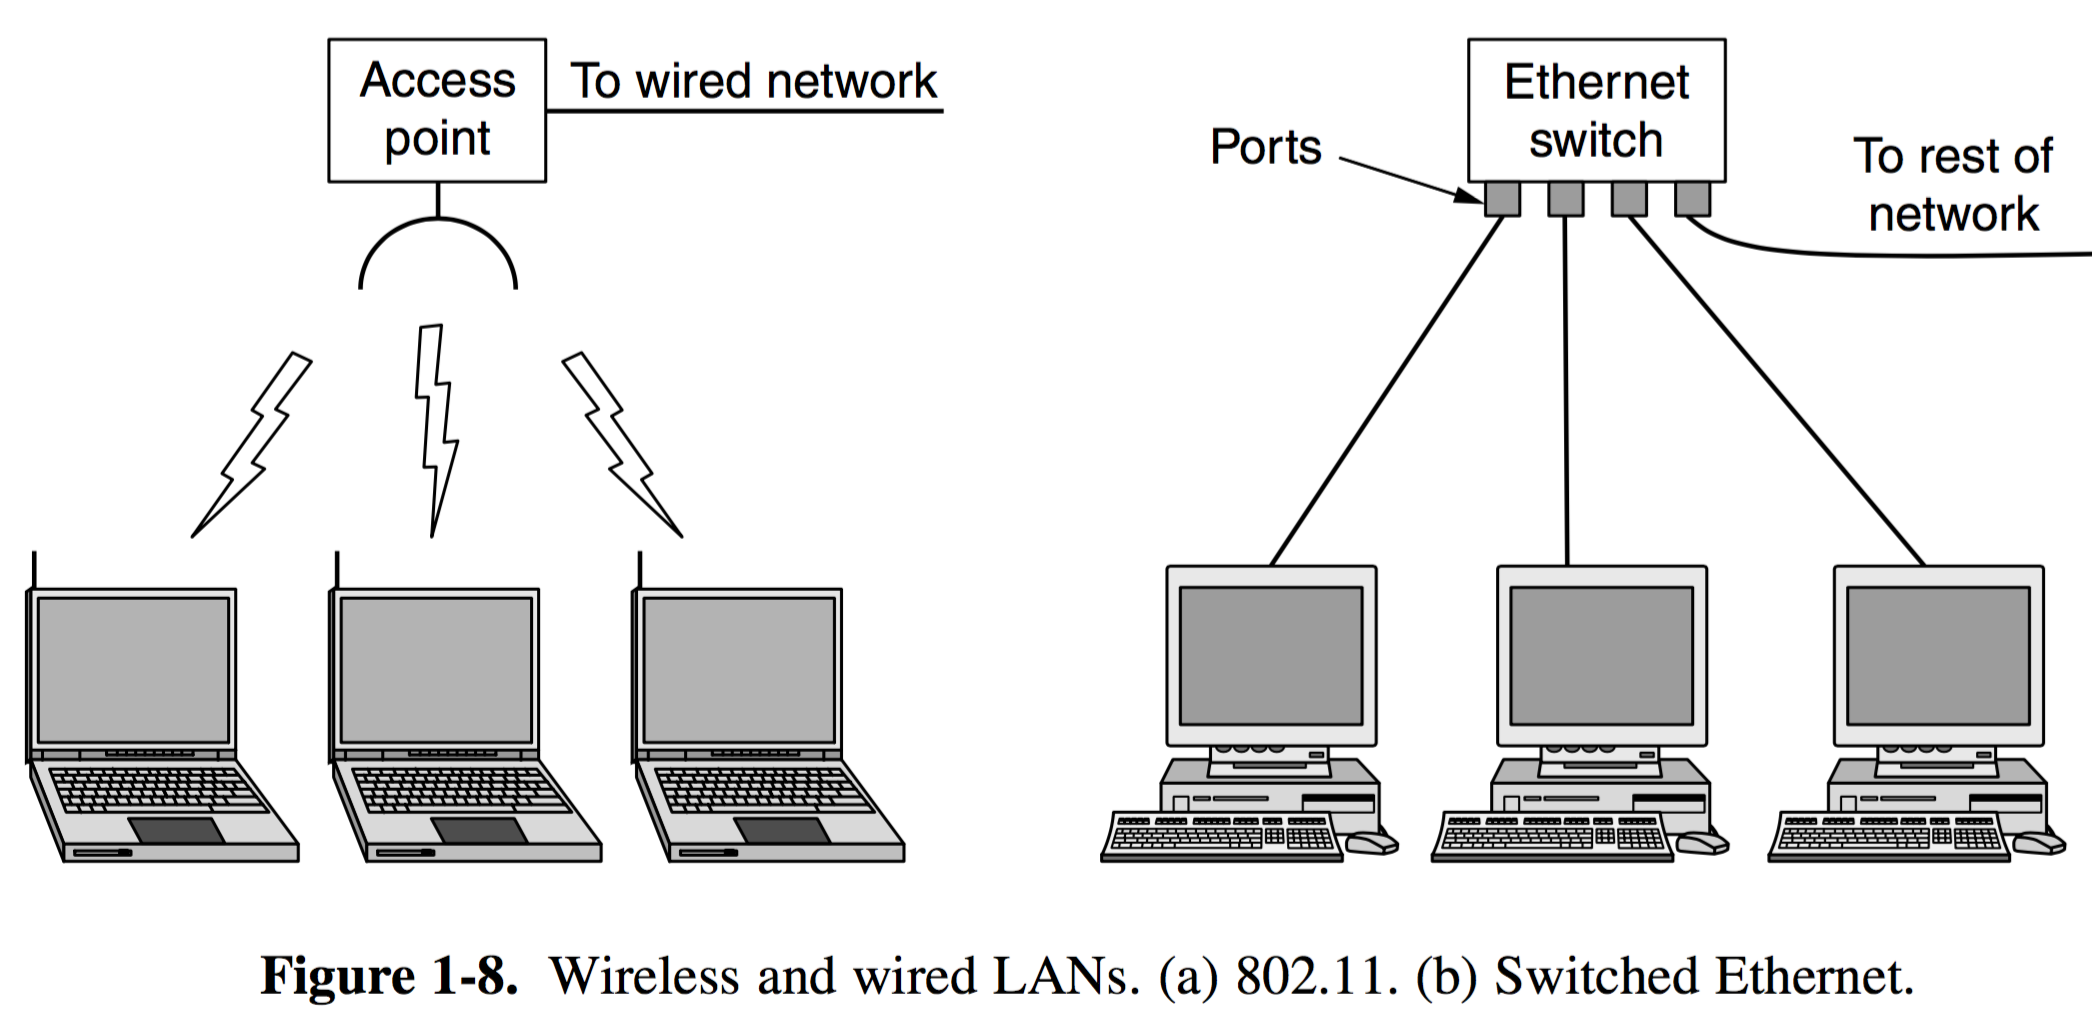
\includegraphics[width=8cm, height=5cm]{./imagenes/arealocal.png} 
\end{center}

\subsection{Redes de área metropolitana}
\par Una Red de área Metropolitana, o MAN (Metropolitan Area Network), cubre toda 
una ciudad.

\textbf{Ejemplo 1:} MAN basada en TV por cable
	\begin{itemize}
		\item Cable coaxil para unir varias casas.
		\item Elementos de conmutación.
		\item Elementos de conmuntación se unen por cables de fibra óptica.
	\end{itemize}
	
	\begin{center}
		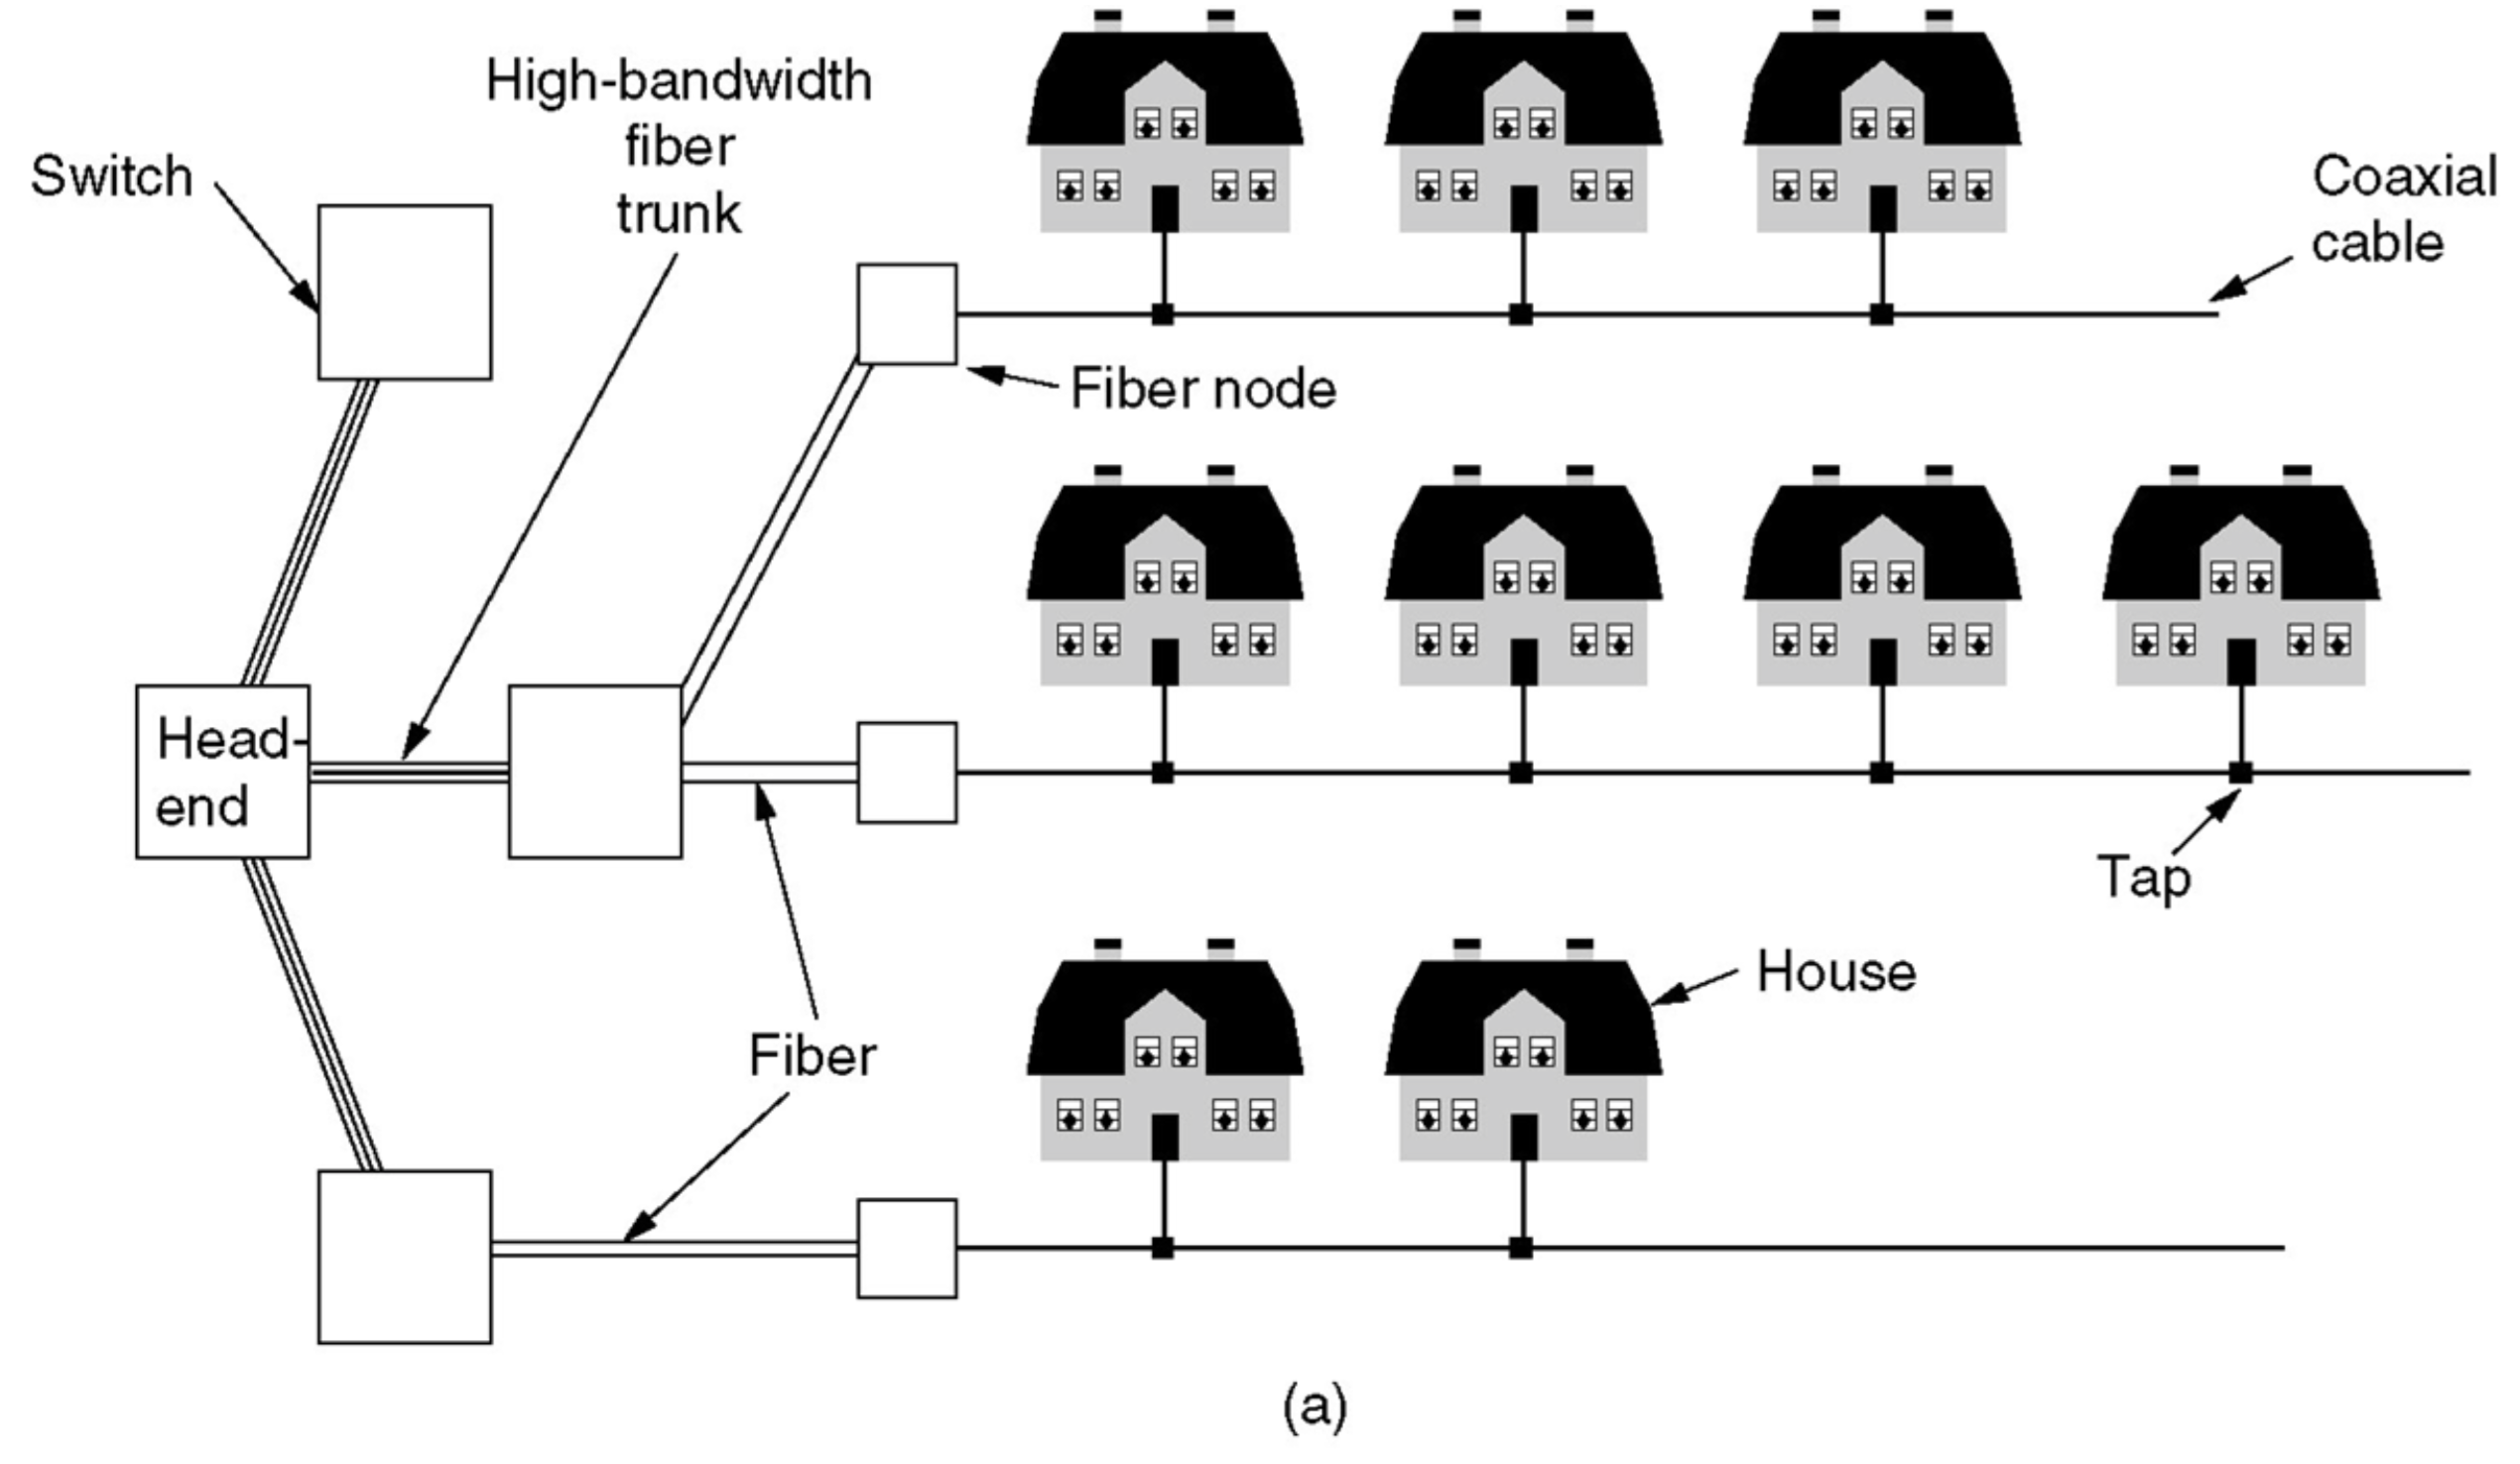
\includegraphics[width=10cm, height=6cm]{./imagenes/metropolitana1.png} 
	\end{center}

\textbf{Ejemplo 2:} Wimax (estándar 802.16).
	\begin{itemize}
		\item Se envían paquetes por el aire en lugar de usar cable o redes telefónicas.
		\item Se conecta a internet (a una red dorsal).
		\item Se puede acceder a la red desde computadoras en casas o edificios, o 
		desde vehículos en movimiento.
	\end{itemize}	 
	
	\begin{center}
		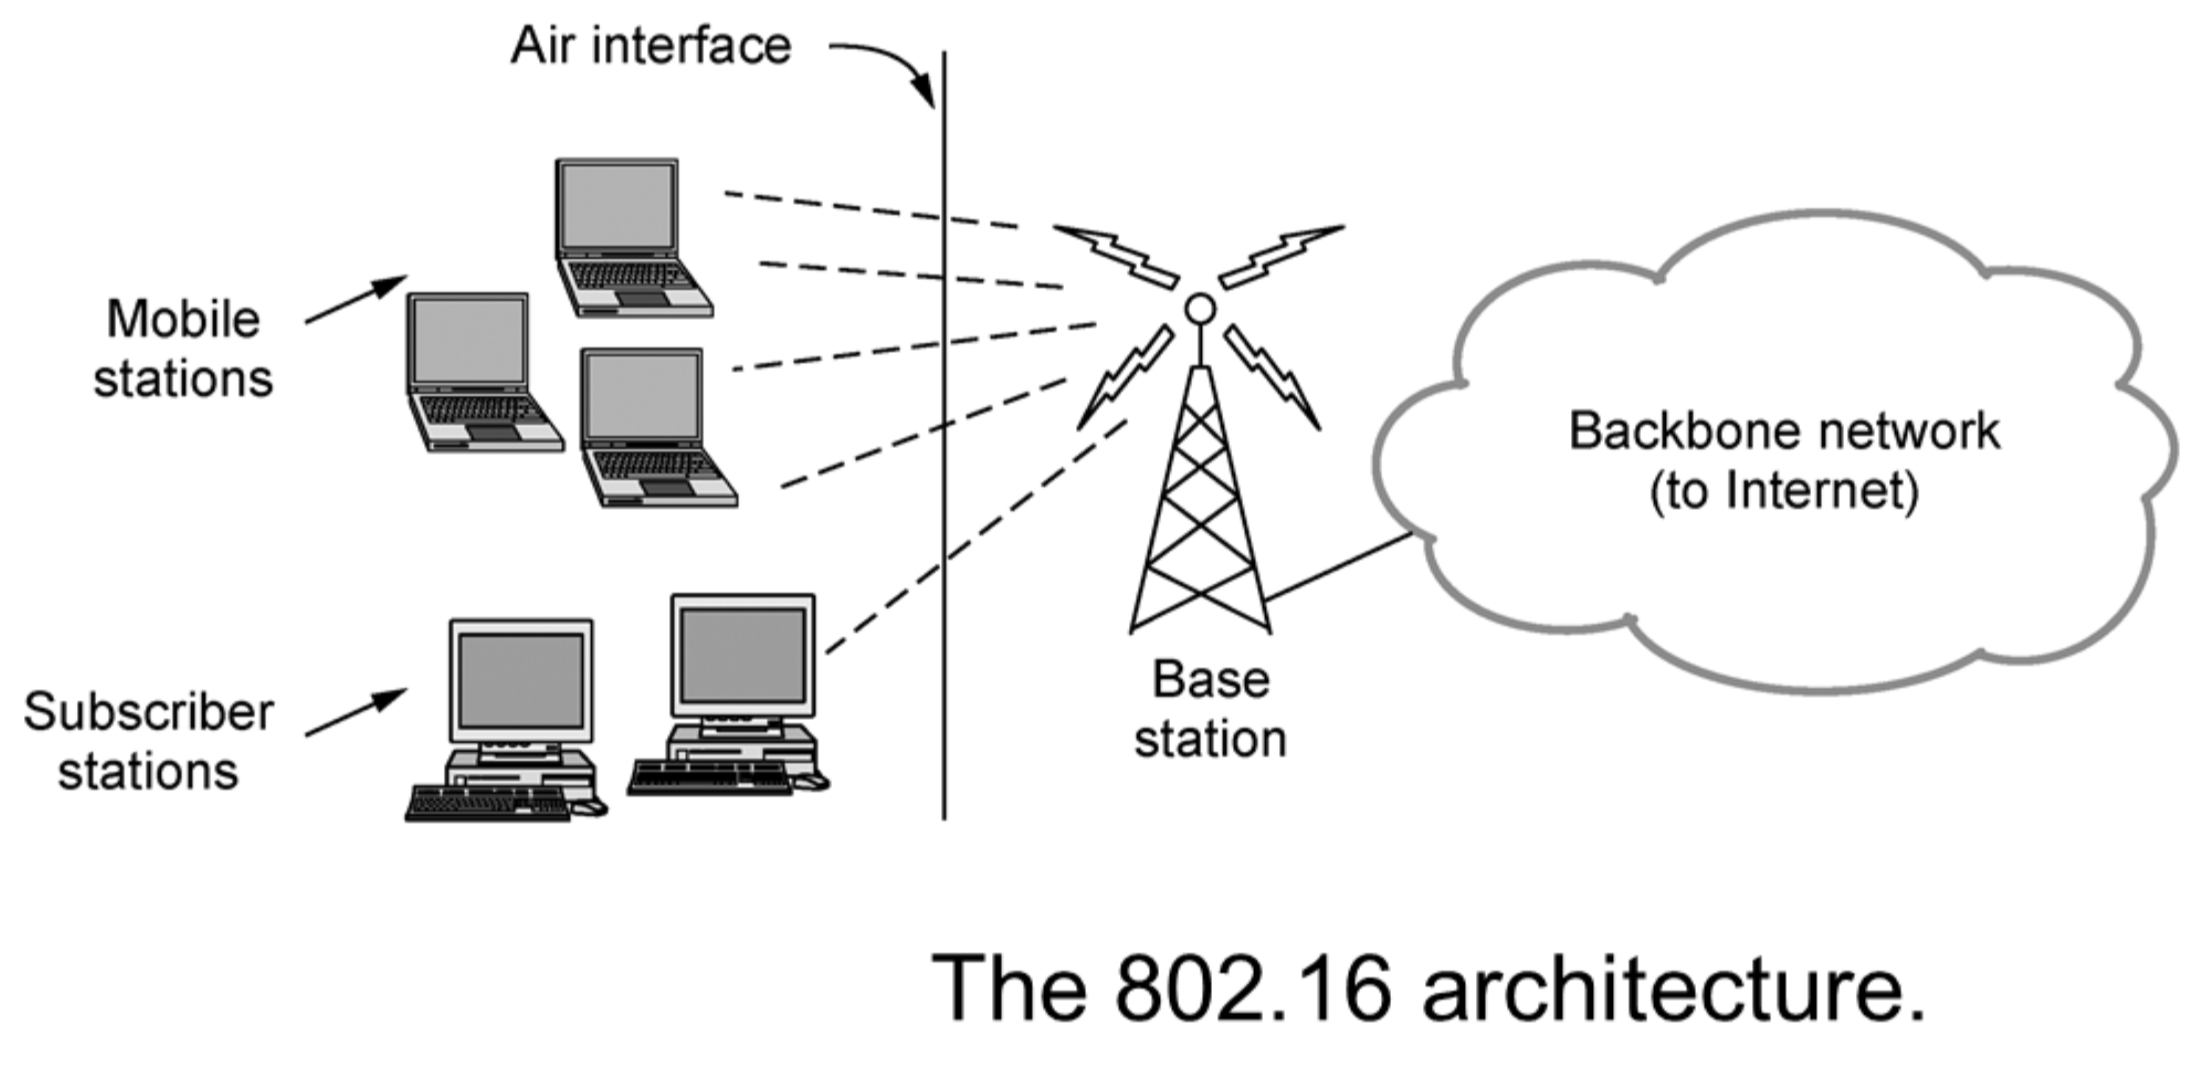
\includegraphics[width=10cm, height=5cm]{./imagenes/metropolitana2.png} 
	\end{center}

\subsection{Redes de área amplia}
\par Una Red de área Amplia, o WAN (Wide Area Network), abarca una extensa área 
geográfica, por lo general un país o continente. Son redes punto a punto: dos 
dispositivos están conectados entre sí por medio de un cable, esta regla da lugar a lo 
que se llama subred.
\par Una \textbf{subred} posee varios enrutadores conectados entre sí formando un 
grafo. A una subred pueden estar conectadas computadoras o redes de área local 
enteras, para ir de una máquina a otra hay distintas rutas alternativas.
\par Los elementos de conmutación, tambien llamados enrutadores dependiendo de la capa de red en la actúan, conectan tres o más líneas de transmisión. Los datos por línea de entrada se envían por alguna línea de salida elegida especialmente.
Dos enrutadores que no comparten una línea de transmisión se conectan indirectamente a través de otros enrutadores.

Un paquete se envía de un enrutador a otro a través de enrutadores intermedios, almacenándose enteramente en cada enrutador intermedio hasta que la línea requerida de salida esté libre y luego se reenvía (\textit{store-and-forward}). Otra forma sería no guardar el mensaje, no esperar a que llegue entero antes de reenviarlo (\textit{cut-through}).

Los mensajes se dividen en paquetes, los cuales tienen un número de secuencia. Estos paquetes se mandan en la red de uno en uno. Los paquetes se van depositando en el host receptor que reensambla el mensaje original. En algunas redes todos los paquetes del mensaje deben seguir la misma ruta, en otras cada paquete se enruta por separado. Las decisiones de enrutamiento se hacen de manera local, un algoritmo de enrutamiento describe la manera en que un enrutador toma esa decisión.

\begin{center} 
	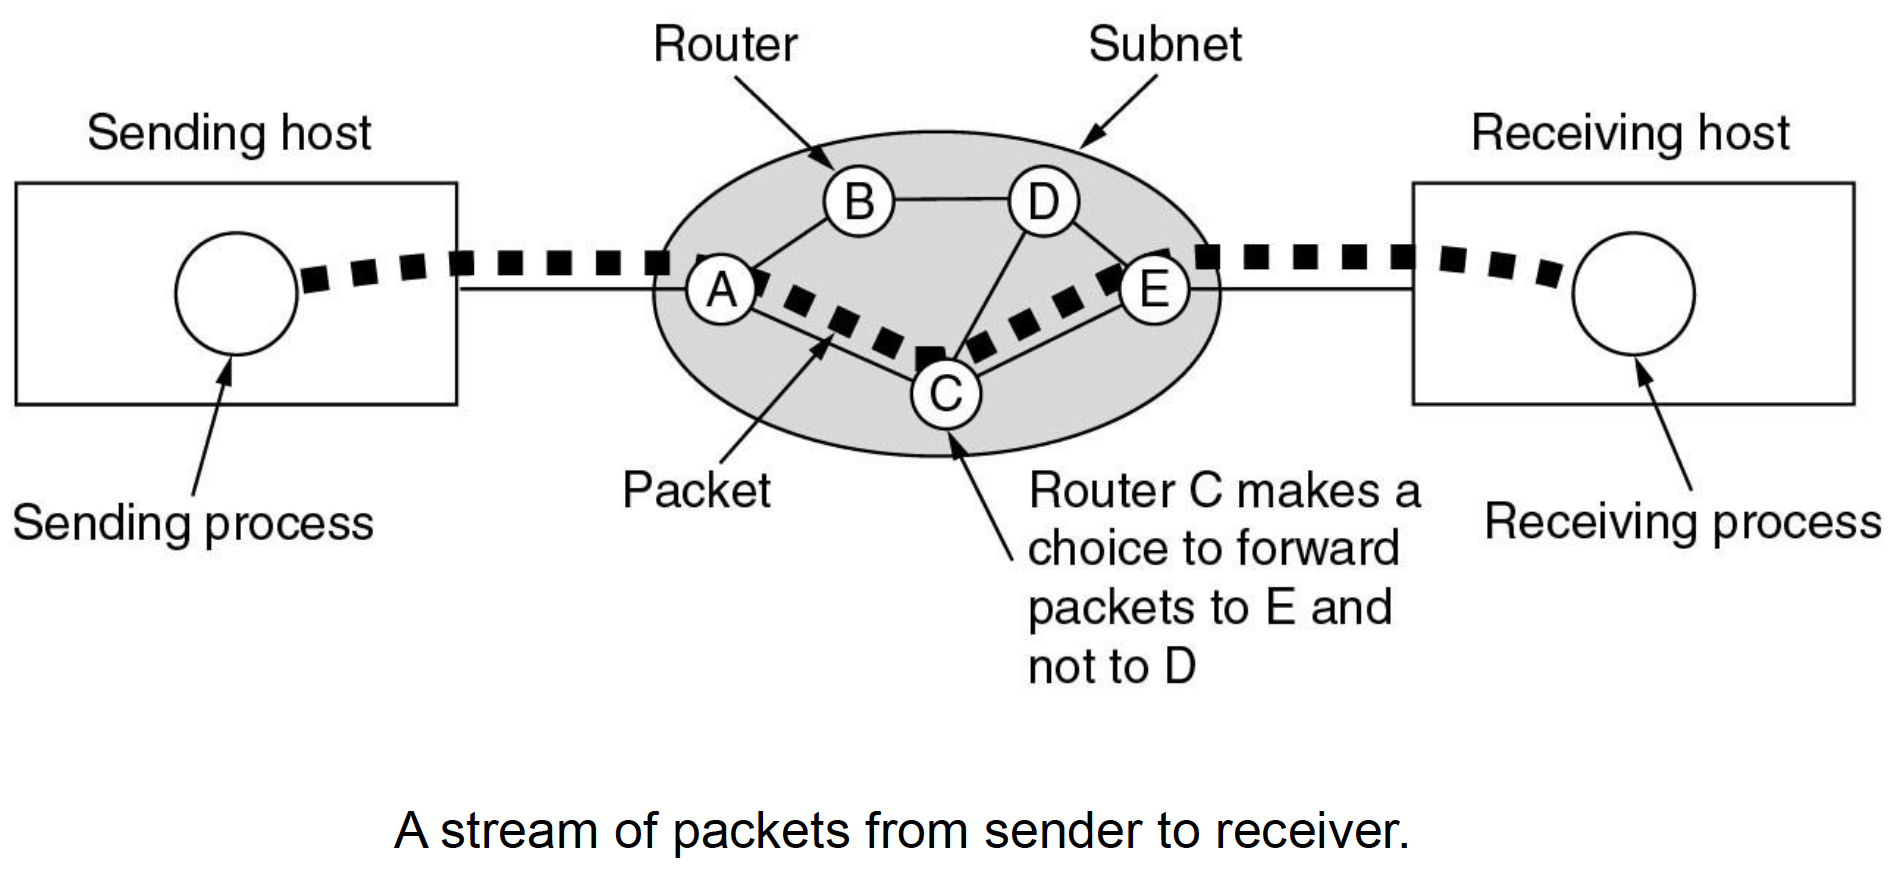
\includegraphics[width=8cm, height=5cm]{./imagenes/wan1.png} 
\end{center}

\subsubsection{Ejemplos de WAN:}
\begin{itemize}
\item Sistema telefónico fijo (Ej: ADSL):
\begin{itemize}
	\item Cada domicilio conectado por un cable de cobre a una End office
 	\item \textit{Toll offices} usadas para reenvío de mensajes.
 	\item \textit{Toll offices} unidas por cables de fibra óptica llamados troncales.
\end{itemize}	

\begin{center} 
	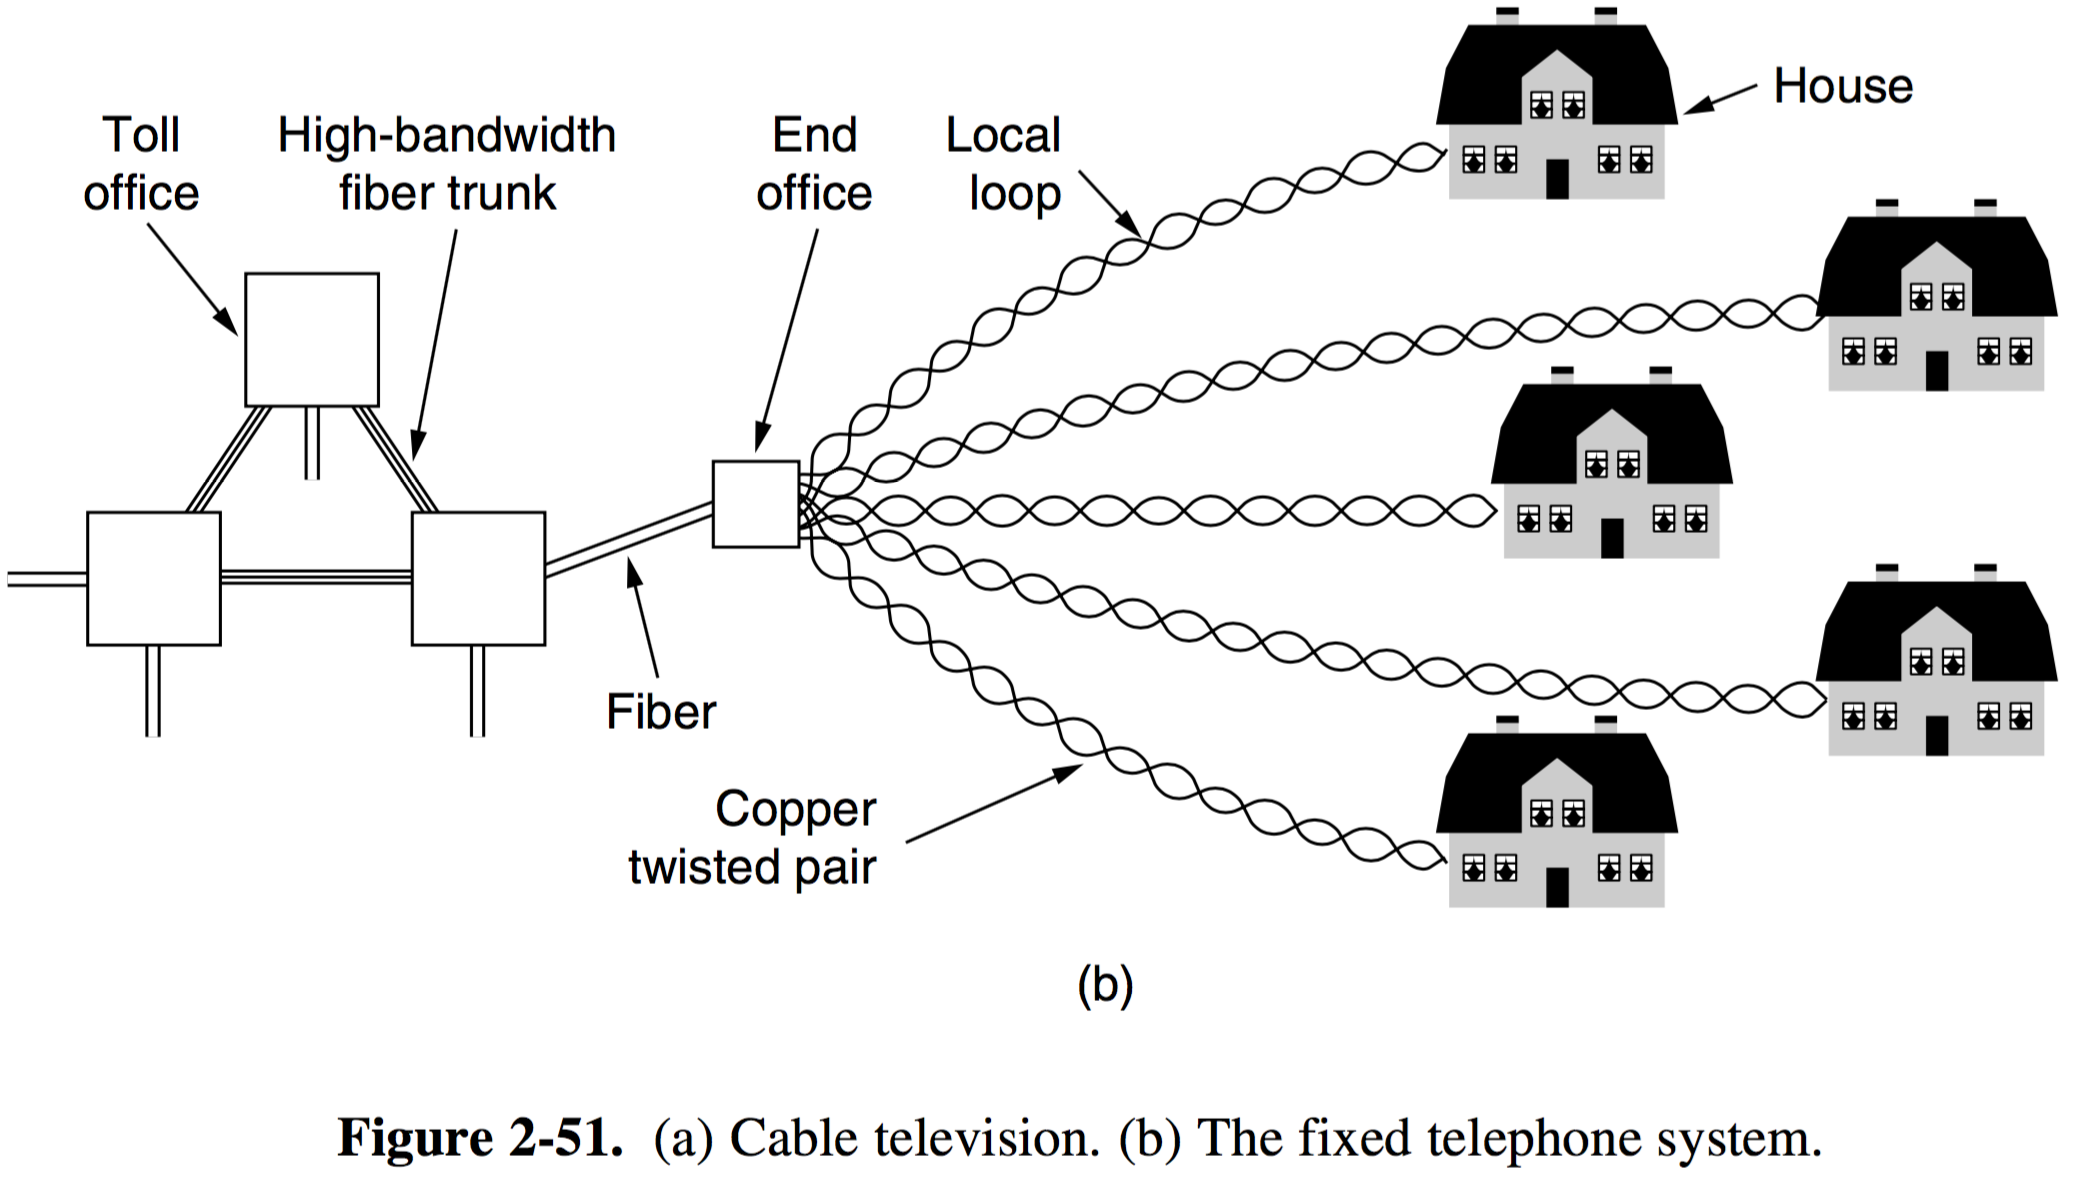
\includegraphics[width=8cm, height=5cm]{./imagenes/telefonico.png} 
\end{center}

\begin{itemize}
	\item Una red de teléfonos celulares (Ej: 3G o 4G).
	\item Celdas con estaciones base: cada smartphone opera en una celda.
	\item Celdas conectados a centros de conmutación: para conectar distintas celdas
 	\item Centros de conmutación conectados a la red telefónica pública.
\end{itemize}

\end{itemize}

\par Un proveedor de servicios de internet (PSI) es también una WAN. Los clientes compran conectividad a un PSI y para usar su red.

\subsection{Interredes}
\par Existen mucha redes en el mundo, a veces con hardware y software diferente. 
Con frecuencia las personas conectadas a una red desean comunicarse con las 
personas conectadas a otra red diferente. Las puertas de enlace proveen la conexión y 
la traducción necesaria. Un conjunto de redes interconectadas se llama interred 
(internet), Internet es una interred.

\begin{center} 
	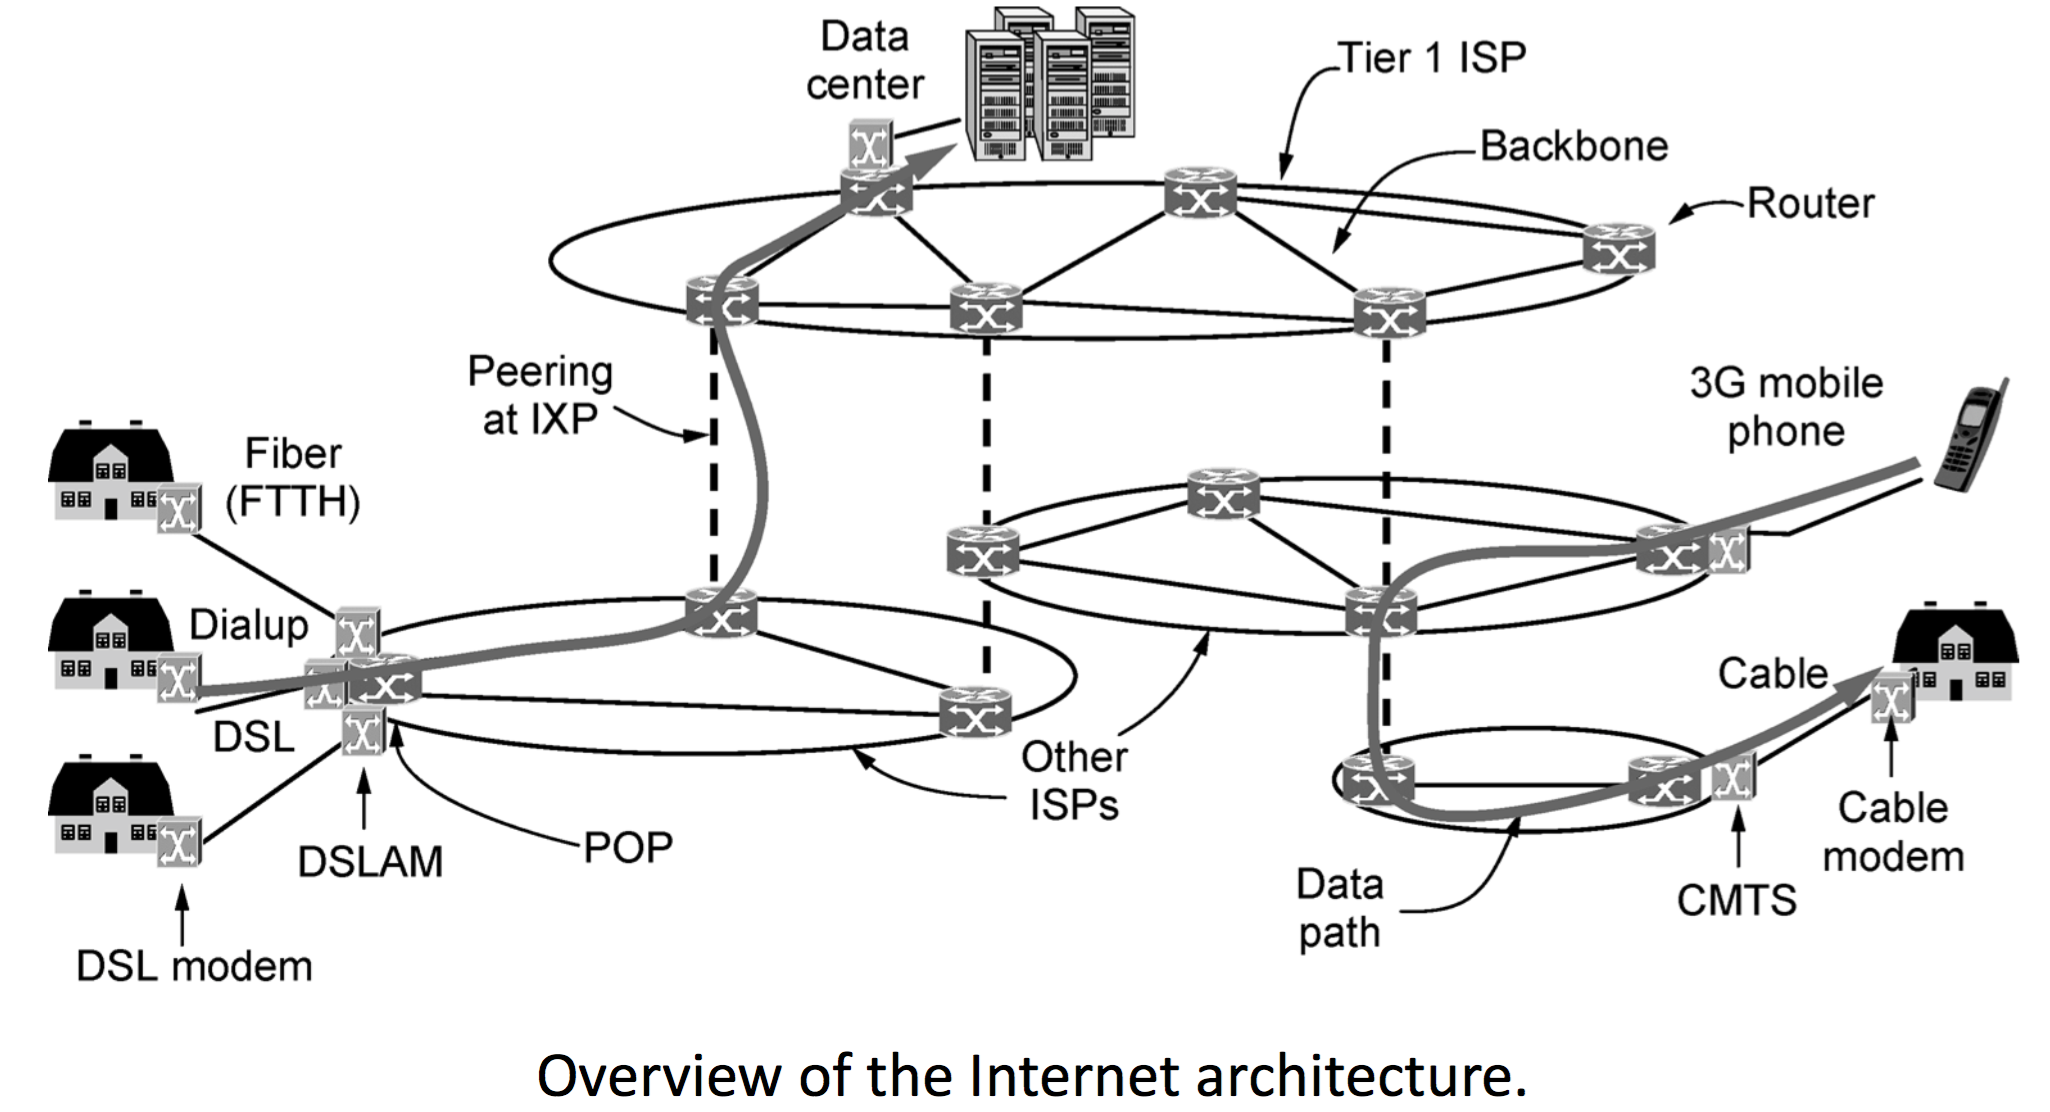
\includegraphics[width=8cm, height=6cm]{./imagenes/interred.png} 
\end{center}

\section{Software de red}
	\par Las primeras redes de computadoras se diseñaron teniendo en cuenta al hardware 
como punto principal y al software como secundario. Pero esta estrategia ya no 
funciona. Ahora el software de red está muy estructurado.

\subsection{Jerarquías de protocolos}
\par Para reducir la complejidad de su diseño, la mayoría de las redes esta organizada 
como una pila de capas o niveles, cada una construida a partir de la que esta debajo de 
ella. El propósito de cada capa es ofrecer ciertos servicios, a las capas superiores, a las 
cuales no se les muestran los detalles de implementación de los servicios ofrecidos. La 
capa \textit{N} de una maquina mantiene una conversación con la capa \textit{N} de 
otra máquina. Las reglas y convenciones utilizadas en esta conversación se conocen 
como \textbf{protocolo de capa N}.
\par Cada capa pasa los datos y la información de control a la capa inmediatamente 
inferior, hasta que se alcanza la capa más baja. Debajo de la capa 1 se encuentra el 
medio físico, a través del cual ocurre la comunicación real. Entre cada par de capas 
adyacentes esta una \textbf{interfaz} que define que operaciones y servicios 
primitivos pone la capa mas baja a disposición de la capa superior inmediata.
\par El conjunto de capas y protocolos se conoce como \textbf{arquitectura de red} o 
\textbf{nomenclatura de pila de protocolos}.

\begin{center} 
	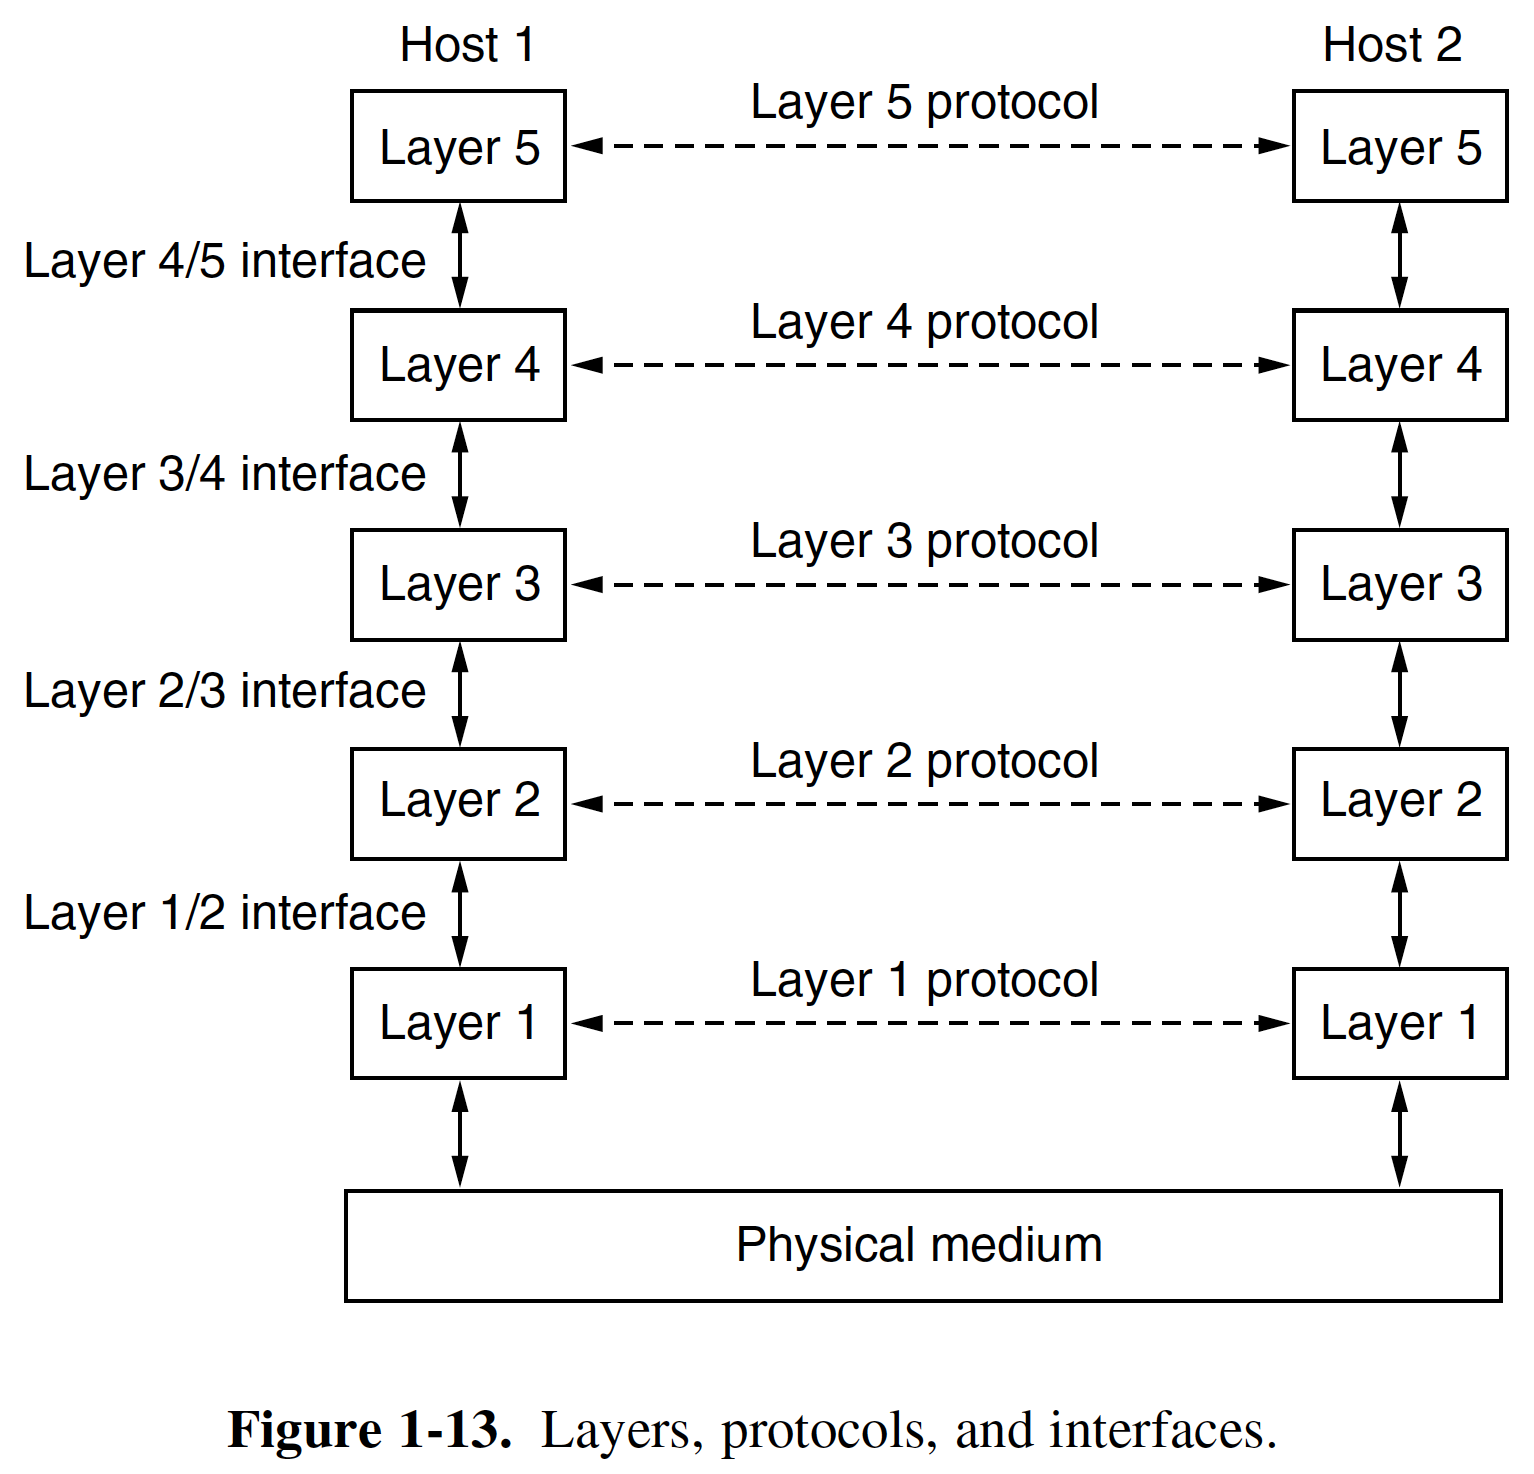
\includegraphics[width=7cm, height=7cm]{./imagenes/jerarquia1.png} 
\end{center}

\par Un proceso de aplicación se ejecuta en la \textit{capa 5}, la cual produce un 
mensaje y lo pasa a la \textit{capa 4} para su transmisión. La \textit{capa 4} pone un 
encabezado en el mensaje para identificarlo y pasa el resultado a la \textit{capa 3}. El 
encabezado contiene información de control como números de secuencia para que la 
\textit{capa 4} de la máquina de destino entregue los mensajes en el orden correcto, 
si las capas inferiores no mantienen la secuencia.

\par En muchas redes no hay limitaciones en el tamaño de los mensajes de la 
\textit{capa 4}, pero casi siempre hay un límite impuesto por el protocolo de la 
\textit{capa 3}, la cual debe dividir  los mensajes que llegan en unidades mas 
pequeñas llamadas \textbf{paquetes} y a cada paquete colocarle un encabezado.
\par La \textit{capa 3} decide cuál de las líneas que salen utilizar y pasa los paquetes 
a la \textit{capa 2} que no solo agrega un encabezado a cada pieza sino tambien un 
terminador, y pasa la unidad resultante a la \textit{capa 1} para su transmisión.
\par En la máquina receptora el mensaje pasa hacia arriba de capa en capa, perdiendo 
los encabezados conforme avanza.

\begin{center} 
	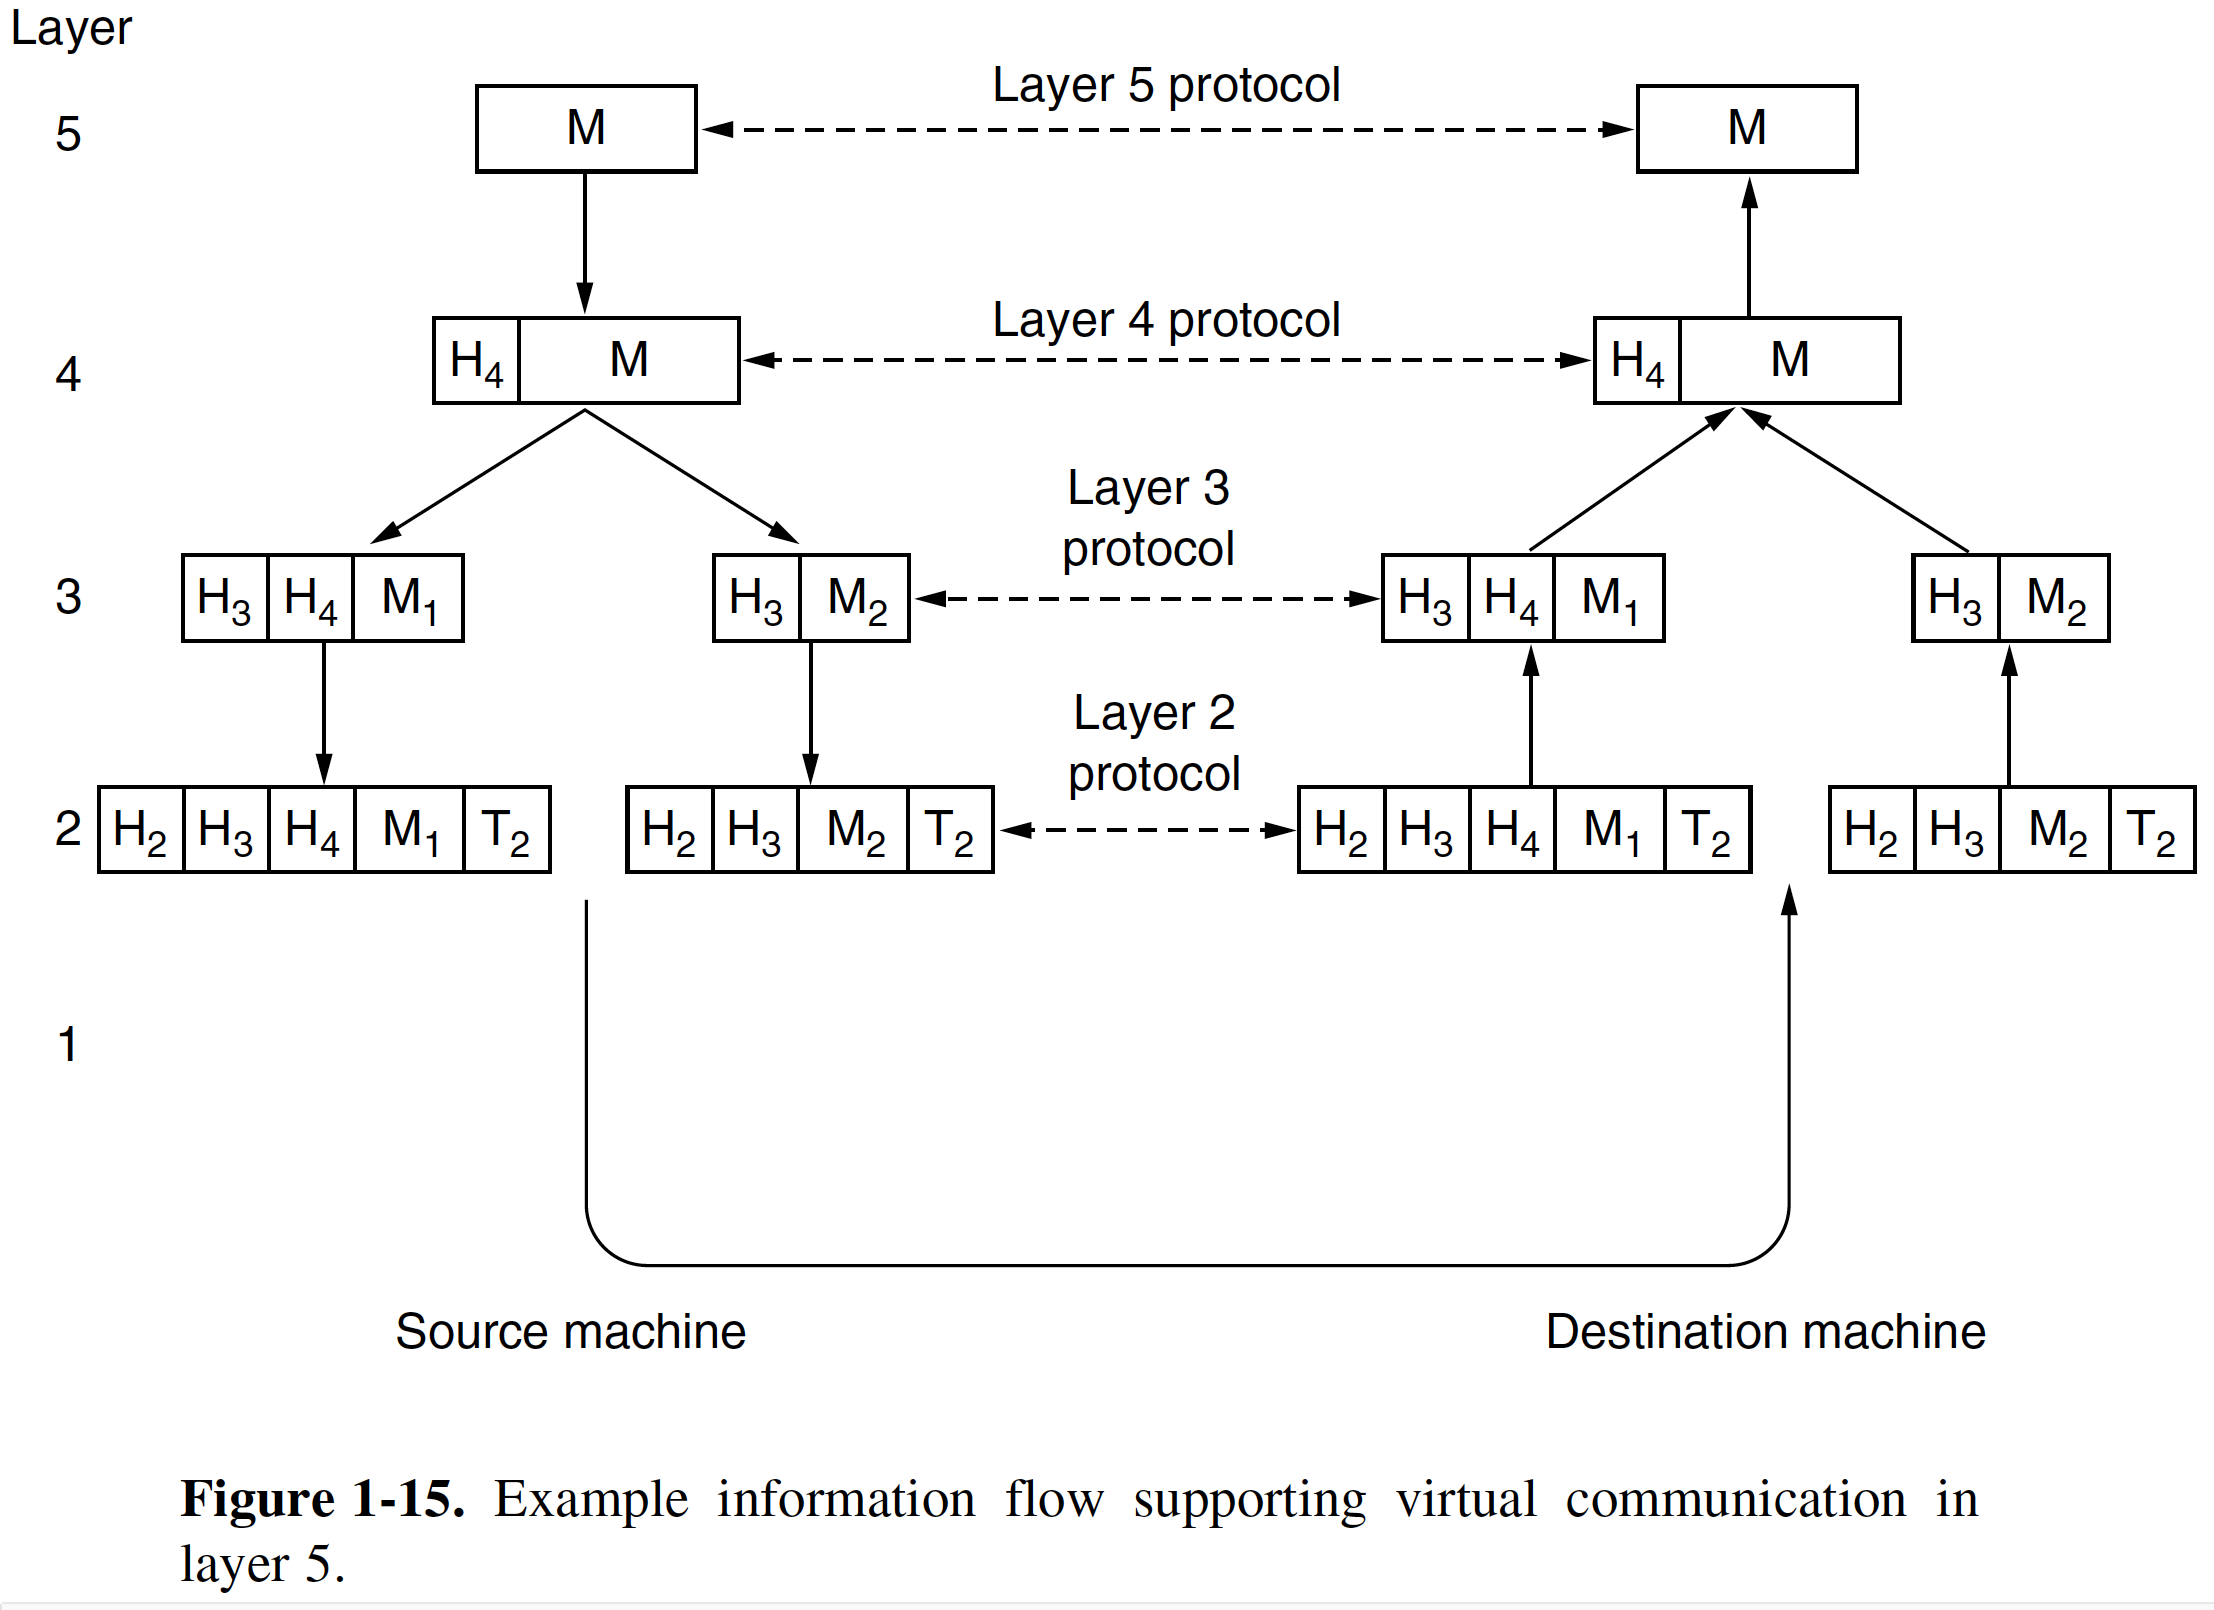
\includegraphics[width=10cm, height=7cm]{./imagenes/jerarquia2.png} 
\end{center}

\subsection{Aspectos de diseño para las capas}

Algunos de los aspectos claves de diseño que ocurren en la redes están presentes en 
las diversas capas, cada capa necesita de un mecanismo para identificar a los emisores 
y a los receptores. Es necesario un método para que un proceso en una máquina 
especifique con cual otra máquina quiere hablar, además de una forma de 
\textbf{direccionamiento} a fin de precisar un destino específico.

\par Otras decisiones de diseño conciernen a las reglas de transferencia de datos, en 
algunos sistemas los datos viajan solo en una dirección, en otros pueden viajar en 
ambas direcciones.

El control de errores es un aspecto importante porque los circuitos de comunicación 
física no son perfectos. Muchos códigos de corrección y detección de errores son 
conocidos, pero los dos extremos de la conexión deben estar de acuerdo en cual es el 
que se va a utilizar. Además, el receptor debe tener algun medio de decirle al emisor 
que mensajes se han recibido correctamente y cuáles no.

\par No todos los canales de comunicación conservan el orden en que se envían los 
mensajes. Para tratar con una posible perdida de secuencia, el protocolo debe incluir 
un mecanismo que permita al receptor volver a unir los pedazos en forma adecuada. 
Una solución obvia es numerar las piezas, pero hay que tratar con las piezas que no 
llegan en orden.

\par Hay que evitar que un emisor rápido sature de datos a un receptor lento. Hay 
soluciones a este problema donde el receptor proporciona algún tipo de 
retroalimentación al emisor, directa o indirectamente, dependiendo de la situación real 
del receptor. A este tema se lo denomina \textbf{control de flujo}. A veces en la red 
demasiadas máquinas quieren enviar demasiados mensajes y la red no puede 
mandarlos a todos, esta sobrecarga se llama \textbf{congestión}. Una solución es que 
cada máquina emisora reduzca el tráfico de salida.

\par En algunos niveles los procesos son incapaces de aceptar mensajes de longitud 
arbitraria. Esta propiedad conduce a mecanismos para desensamblar, transmitir y 
reensamblar mensajes. A este tema en general se lo conoce como 
\textbf{interconexión de redes}.

\par Cuando es costoso mantener una conexión separada para cada par de procesos 
de comunicación, la capa subyacente podría decidir usar la misma conexión para 
múltiples conversaciones sin relación entre si, siempre y cuando esta 
\textbf{multiplexión} y demultiplexión se realice de manera transparente, cualquier 
capa la podrá utilizar. La multiplexión se necesita en la capa física, donde múltiples 
conversaciones comparten un número limitado de circuitos físicos.

\par Cuando hay múltiples rutas entre el origen y el destino se debe elegir la mejor o 
las mejores entre todas ellas, este tema se llama \textbf{enrutamiento}.

\subsection{Comparación entre servicio orientado a conexión y servicio sin conexión}
\par Normalmente una capa puede ofrecer distintos tipos de servicio a las capas arriba 
suyo. El servicio orientado a la conexión, el usuario del servicio primero establece una 
conexión, la utiliza y luego la abandona. Una conexión funciona como un tubo: el 
emisor empuja objetos en un extremo y el receptor los toma en el otro extremo. Se 
conserva el orden en que esos objetos salen y llegan.
\par En el servicio no orientado a la conexión cada mensaje lleva completa la dirección 
de destino y cada uno se enruta a través del sistema, independientemente de los 
demás. Algunos servicios son confiables en el sentido que nunca pierden datos, pero 
por lo general en un servicio confiable el receptor confirma la recepción de cada 
mensaje. Al servicio no orientado a la conexión no confiable, es decir sin confirmación 
de recepción, se lo conoce como \textbf{servicio de datagramas}. 
\par A veces se desea no tener que establecer una conexión para enviar un mensaje 
corto, pero la confiabilidad es esencial. Para estas aplicaciones se usa el servicio de 
\textbf{datagramas confirmados}. En el servicio de \textbf{solicitud-respuesta} el 
emisor transmite un solo datagrama con una solicitud y luego el receptor envía la 
respuesta al estilo del modelo cliente-servidor.


\section{Modelos de referencia}

\subsection{El modelo de referencia OSI}

\subsubsection{La capa de enlace de datos}
\par La tarea principal de la capa de enlace de datos es transformar un medio de 
transmisión puro en una línea de comunicación que aparezca libre de errores de 
transmisión. El emisor fragmenta los datos de entrada en \textbf{tramas de datos}, y 
transmite las tramas de manera secuencial. Si el servicio es confiable, el receptor 
confirma la recepción correcta de cada trama devolviendo una \textbf{trama de 
confirmación de recepción}.
\par Otro problema atacado es como hacer que un emisor rápido no sature de datos a 
un receptor lento: mecanismo de regulación de tráfico. Con frecuencia esta regulación 
de flujo y el manejo de errores están integrados. Las redes de difusión además 
consideran como controlar el acceso a un canal compartido. La subcapa de control de 
acceso al medio se ocupa de esto.

\subsubsection{La capa de red}
\par La capa de red controla las operaciones de la subred. Hay que determinar cómo se enrutan los paquetes desde su origen a su destino. Si hay demasiados paquetes en la subred al mismo tiempo, se interpondrán en el camino unos y otros lo que hará que se formen cuellos de botella, la capa de red se ocupa de controlar esta congestión.
\par Cuando un paquete tiene que viajar de una red a otra para llegar a destino pueden surgir varios problemas; el direccionamiento de la segunda red podría ser distinto, la segunda podría no aceptar el paquete porque es demasiado largo, los protocolos podrían ser distintos, etc. La capa de red resuelve estos problemas.

\subsection{El modelo de referencia TCP/IP}

	\par Se eligió una red de conmutación de paquetes basada en una capa de interred no 
orientada a la conexión. El trabajo de la capa de interred es permitir que los \textit{hosts} inyecten paquetes dentro de cualquier red y que estos viajen a su destino de manera independiente. Tal vez lleguen en un orden distinto al cual fueron enviados, en cuyo caso las capas mas altas deberán ordenarlos, si se desea una entrega ordenada. La capa de interred define un paquete de formato y protocolo oficial llamado IP (\textit{protocolo de internet}).

	\par \textbf{Direcciones IP:} compuestas por 4 números entre 0 y 255 separados por un punto . Ej: 200.45.191.35. El trabajo de la capa de interred es entregar paquetes IP al destinatario. El enrutamiento de paquetes es el aspecto principal, con el propósito de evitar la congestión.

 	\par La capa arriba de la capa interred es la capa de transporte, la cual esta diseñada para permitir que las entidades iguales en los hosts de origen y destino puedan llevar a cabo una conversación. Se tienen dos protocolos de transporte:

	\begin{itemize}
		\item \textbf{TCP:} es confiable, orientado a la conexión y permite que un flujo de bytes que se origina en una máquina se entregue sin errores en cualquier otra máquina en la interred. Divide el flujo en de bytes entrantes en mensajes discretos y pasa cada uno de ellos a la capa de interred. En el destino el proceso TCP receptor reensambla en el flujo de salida los mensajes recibidos. TCP también maneja el control de flujo para que un emisor rápido no sature con mas mensajes que los que puede manejar a un receptor lento.
		\item \textbf{UDP} es un protocolo no confiable y no orientado a la conexión, para aplicaciones que no desean el control de flujo ni la secuenciación de mensajes. Tiene un amplio uso en consultas de solicitud-respuesta de tipo cliente-servidor en un solo envío y en aplicaciones de transmisión de voz y video.
	\end{itemize}

	\par La capa de aplicación contiene todos los protocolos de nivel mas alto: terminal virtual (TELNET), transferencia de archivos (FTP), correo electrónico (SMTP), para resolución de nombres de host en sus direcciones de red (DNS), para páginas web (HTTP).

	\begin{center}
		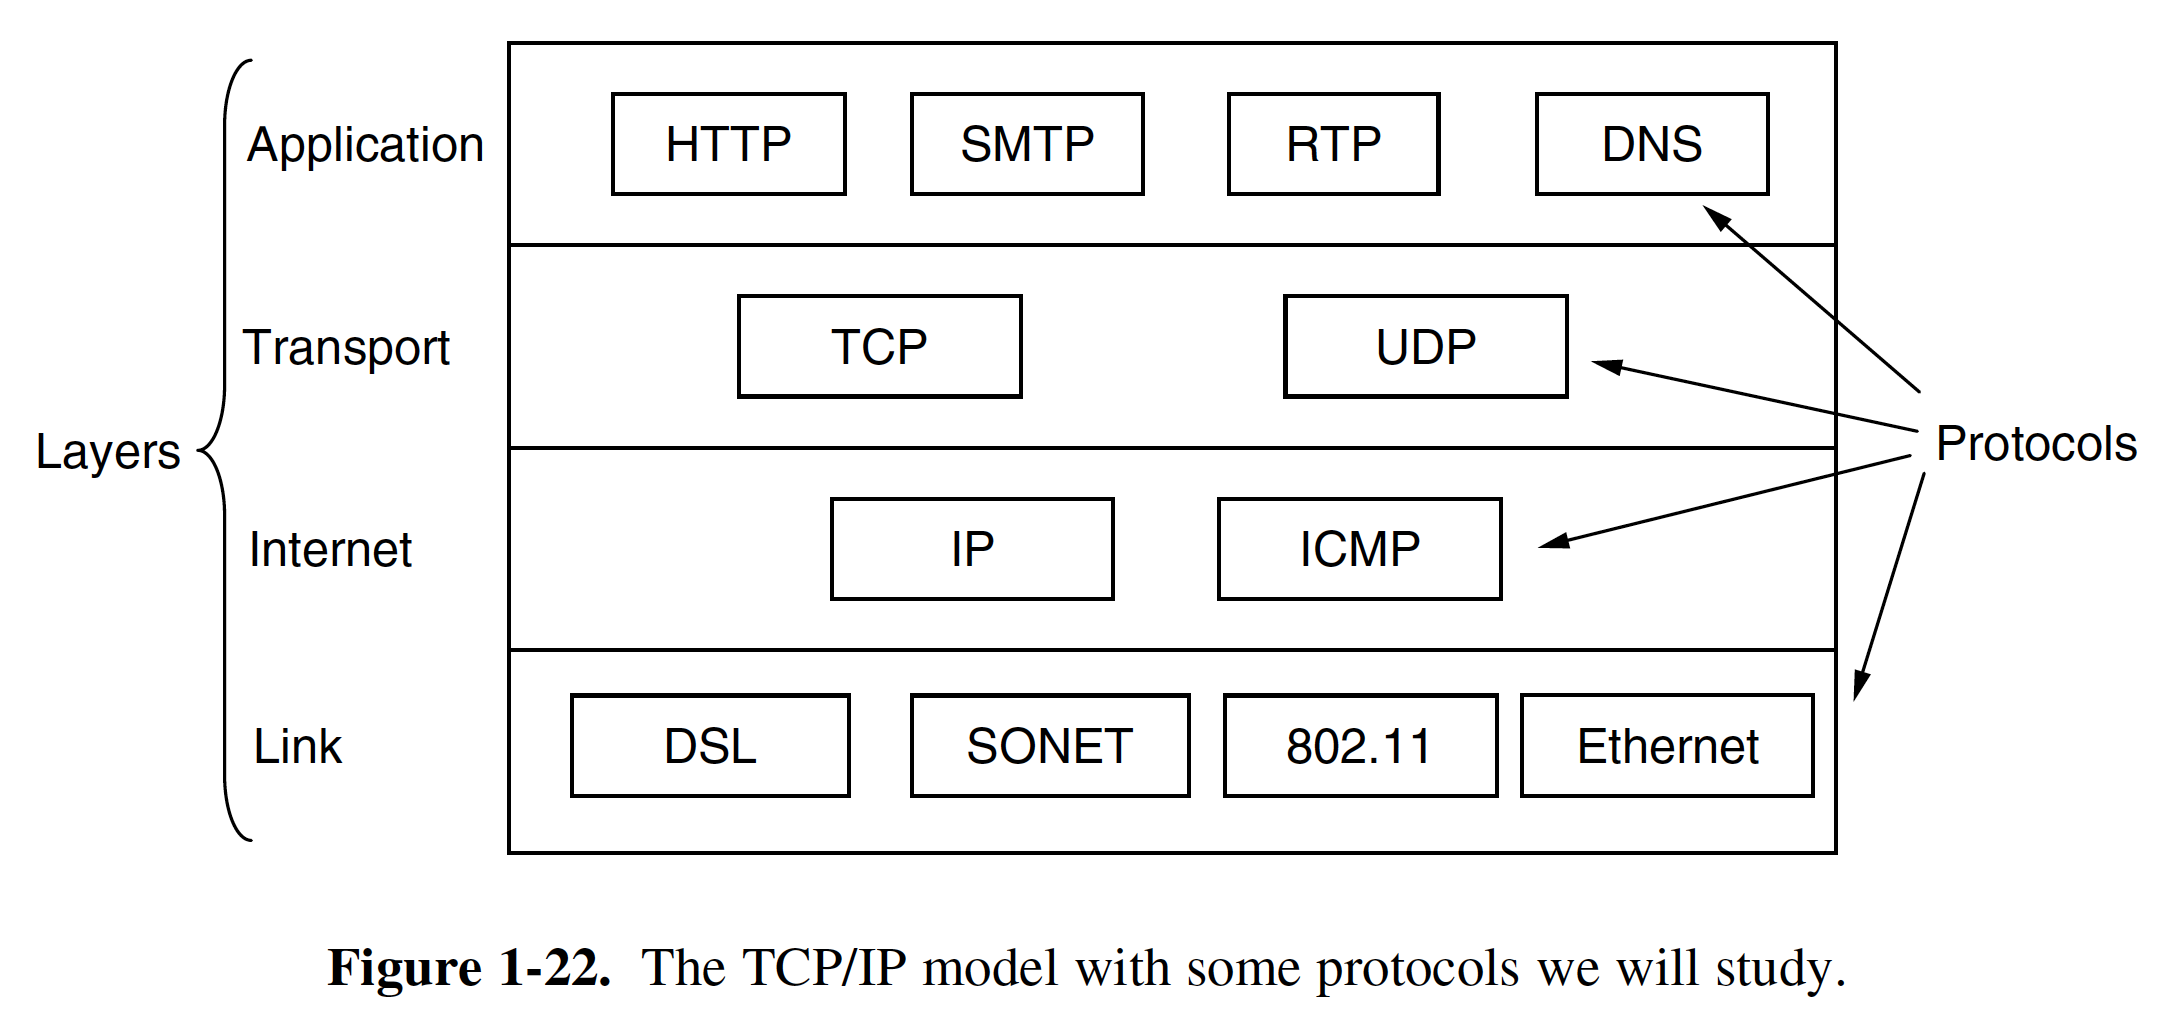
\includegraphics[width=11cm, height=5cm]{./imagenes/esquema.png} 
	\end{center}
	
\subsection{Una crítica al modelo de referencia TCP/IP}

	\par El modelo TCP/IP tiene problemas, alguna de ellos son: No se distingue entre servicio, interfaz y protocolo, o sea no se distingue bien entre especificación e implementación. No es un modelo general no está ajustado para describir ninguna pila de protocolos mas que TCP/IP. No se mencionan las capas físicas y de enlace de datos. Protocolos altamente entrincherados y difíciles de remplazar.

\section{Redes de ejemplo}

\subsection{Internet}
\par Internet es un inmenso conjunto de redes diferentes, que usan ciertos protocolos comunes y proporcionan ciertos servicios comunes. A este sistema nadie lo planeo y nadie lo controla. 

\par Los protocolos TCP e IP están preparados para manejar comunicaciones por 
interredes. Se desarrollo una interfaz de programación para la red llamada sockets 
de Berkeley.

	\par Luego se creo el DNS (sistema de nombres de dominios) para organizar máquinas 
dentro de dominios y resolver nombres de \textit{hosts} en direcciones IP. Una máquina esta en Internet si ejecuta una pila de protocolos TCP/IP, tiene una dirección IP y puede enviar paquetes a todas las demás maquinas de Internet. Muchas máquinas pueden llamar a un proveedor de servicios de Internet mediante un modem, recibir direcciones IP temporales y enviar paquetes a otros hosts de Internet.

\section{Modelo Hibrido}

	\begin{center}
		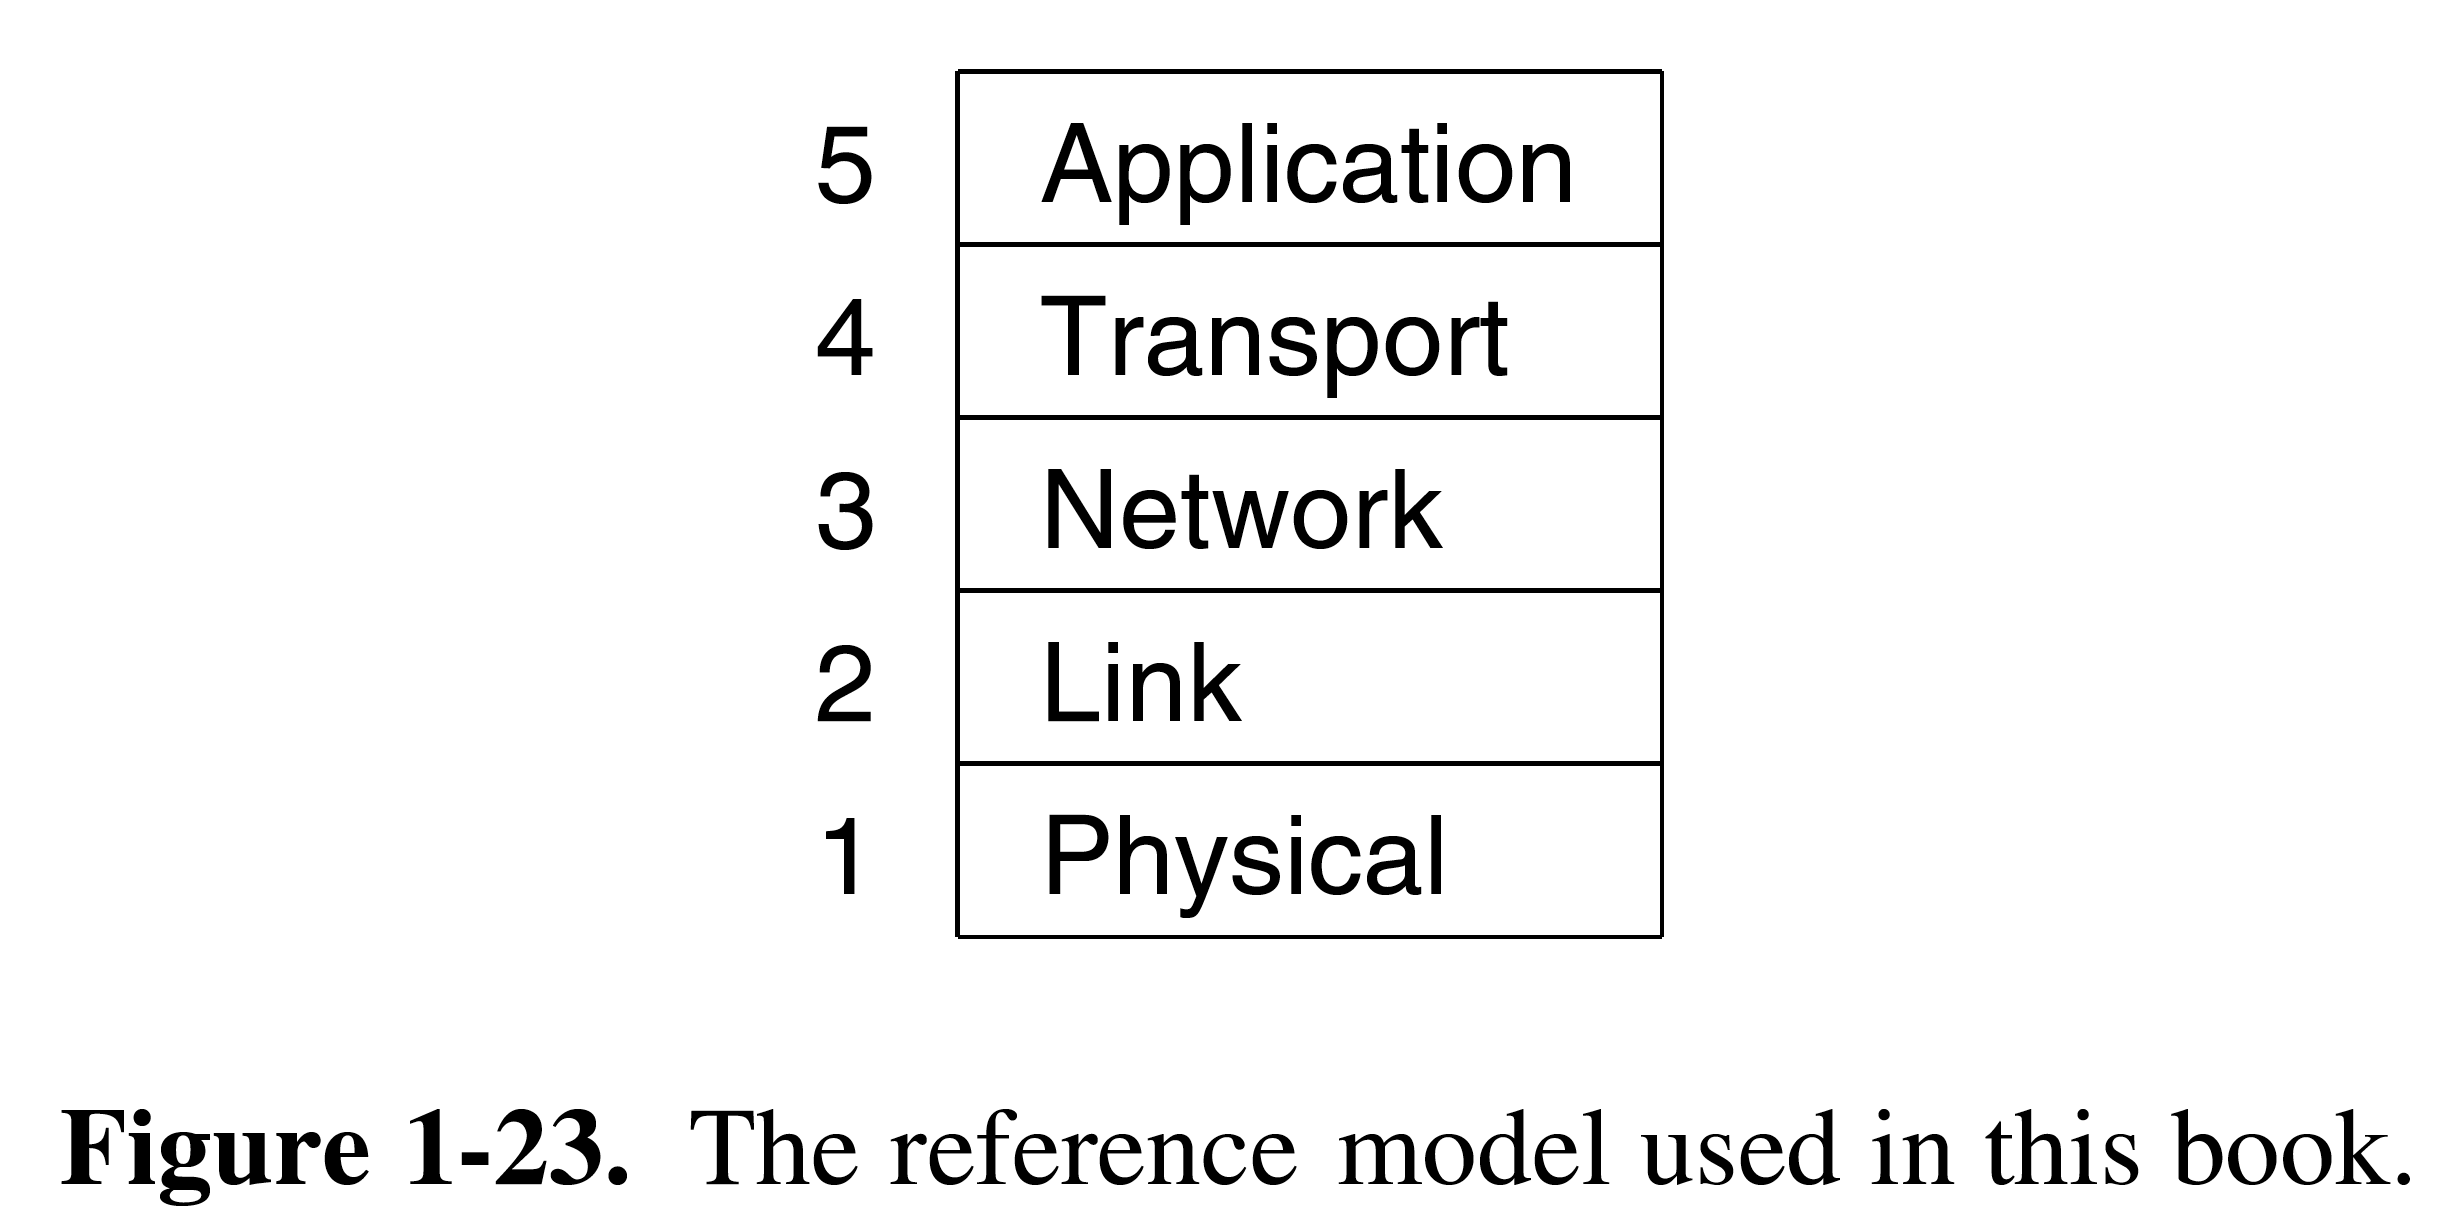
\includegraphics[width=8cm, height=5cm]{./imagenes/modelo.png} 
	\end{center}
